% Latex File for Computer Vision Coursework 2
\documentclass[a4paper]{article}

% Packages
\usepackage{hyperref}
\usepackage[a4paper, total={6.5in,10in}]{geometry}
\usepackage{multicol,caption}
\setlength{\columnsep}{1cm}
\usepackage{courier}
\usepackage{graphicx}
\newenvironment{Figure}
{\par\medskip\noindent\minipage{\linewidth}}
{\endminipage\par\medskip}
\usepackage[toc,page]{appendix}

% Code Package
\usepackage[utf8]{inputenc}
\usepackage{listings}
\usepackage{color}
\definecolor{codegreen}{rgb}{0,0.6,0}
\definecolor{codegray}{rgb}{0.5,0.5,0.5}
\definecolor{codepurple}{rgb}{0.58,0,0.82}
\definecolor{backcolour}{rgb}{0.95,0.95,0.92}
\definecolor{mygreen}{RGB}{28,172,0} % color values Red, Green, Blue
\definecolor{mylilas}{RGB}{170,55,241}
\lstdefinestyle{mystyle}{
	backgroundcolor=\color{backcolour},   
	commentstyle=\color{codegreen},
	keywordstyle=\color{magenta},
	numberstyle=\tiny\color{codegray},
	stringstyle=\color{codepurple},
	basicstyle=\footnotesize,
	breakatwhitespace=false,         
	breaklines=true,                 
	captionpos=b,                    
	keepspaces=true,                 
	numbers=left,                    
	numbersep=5pt,                  
	showspaces=false,                
	showstringspaces=false,
	showtabs=false,                  
	tabsize=2
}
\lstset{style=mystyle}
\setlength{\parindent}{0cm}

% MATLAB template
\lstset{language=Matlab,%
	%basicstyle=\color{red},
	breaklines=true,%
	morekeywords={matlab2tikz},
	keywordstyle=\color{blue},%
	morekeywords=[2]{1}, keywordstyle=[2]{\color{black}},
	identifierstyle=\color{black},%
	stringstyle=\color{mylilas},
	commentstyle=\color{mygreen},%
	showstringspaces=false,%without this there will be a symbol in the places where there is a space
	numbers=left,%
	numberstyle={\tiny \color{black}},% size of the numbers
	numbersep=9pt, % this defines how far the numbers are from the text
	emph=[1]{for,end,break},emphstyle=[1]\color{red}, %some words to emphasise
	%emph=[2]{word1,word2}, emphstyle=[2]{style},    
}

\title{COMP3200: Individual Project \\ Reinforcement Learning}
\author{Daniel Lee \\ \href{emailto: dl2g14@ecs.soton.ac.uk}{dl2g14@ecs.soton.ac.uk}}


\begin{document}
	\maketitle
	
	\begin{multicols}{2}[
		\section*{Motivation}
		The purpose of this paper is to document every relevant work that I do during my background research.
		]
		
		\section{Bandit Problems}
		In the classic bandit problem, the agent is given a limited set of actions to choose from at every time-step. Each action provides the agent with its respective stochastic reward from a particular distribution. The objective is to collect as much total reward, or \textit{return}, from the limited amount of available time-steps. In this section, the popular greedy and $\epsilon$-greedy algorithms will be implemented to tackle this task and the resulting performances will be compared.

		\subsection{Greedy}
		\subsubsection{Theory}
		As mentioned above, the agent can choose an action from a limited range of options. The greedy algorithm leads the agent to choose the action that has the highest \textit{action-value} at every single time-step. This can be numerically represented in this way: 
		
		\begin{equation}
			Q_t(A_t^*) = max_a Q_t(a)
		\end{equation}
		
		The action-value of an action can be computed from the following equation (2):
		
		\begin{equation}
			Q_t(a) = \frac{R_1 + R_2 + ... + R_{K_a}}{K_a}
		\end{equation}

		The equation states that the action-value of an action at a particular time-step is determined by the total reward accumulated, divided by the number times that it was selected in the past. In this simulation, the probability distribution that was used for the immediate actions' rewards was a Gaussian distribution $\mathcal{N}$(0,1). Due to the nature of this distribution, if an action was selected infinite times, its action-value would eventually converge to its \textit{actual} value, $q_*$.
		
		\subsubsection{Simulation}
		To test this algorithm, the \textit{actual} values for each of the actions were set by selecting numbers from a $\mathcal{N}$(0,1) distribution. Following this, the action-values were initialized by adding Gaussian noise of the form $\mathcal{N}$(0,1). To test the performance of the greedy algorithm, the simulation was first run for 300 steps from a bandit problem with 5 possible actions and averaged over 300 bandits. In Figure (1), we can see the average return from simulating an 5-bandit problem with a range of 5 actions over 300 steps.
		
		\begin{Figure}
			\centering
				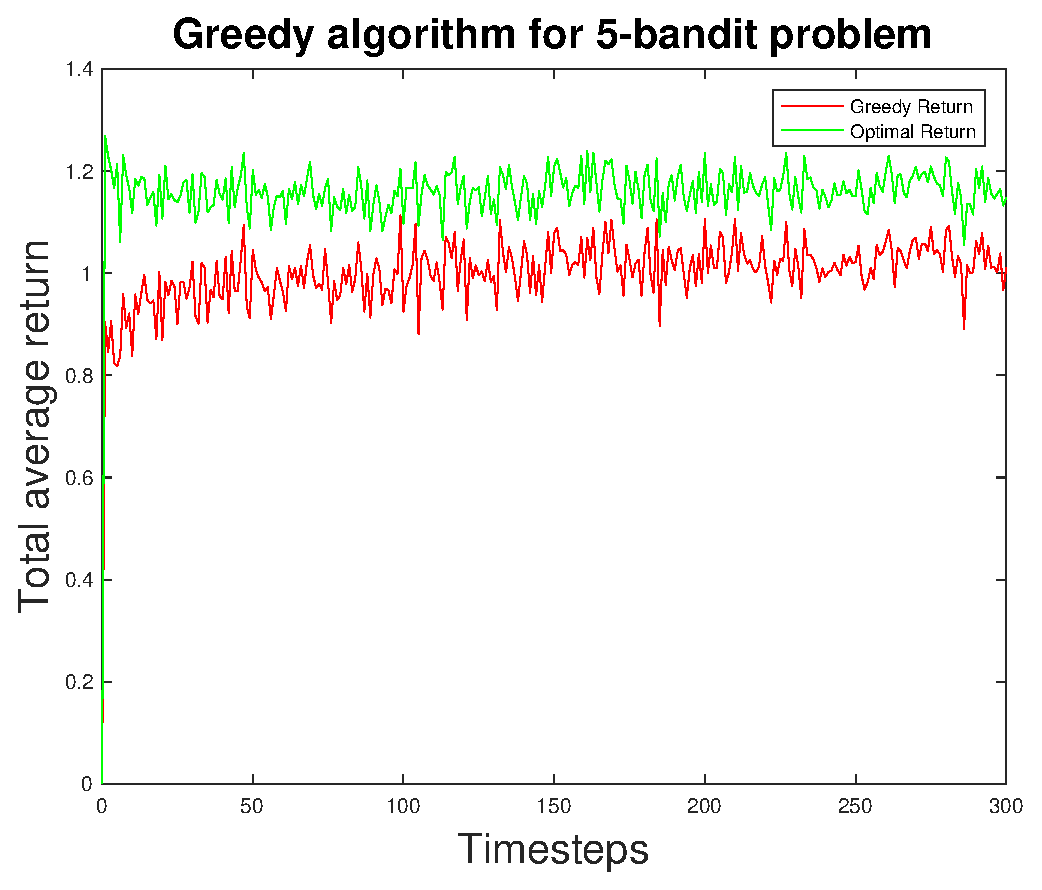
\includegraphics[width=\linewidth]{greedyplot1.eps}
			\captionof{figure}{Greedy vs Optimal}
		\end{Figure}
		
		It can be observed that the greedy method performs around 0.2 worse than the optimal solution in average. A better way of analyzing the performance of the greedy algorithm can be computed by observing the percentage of the times that the agent chose the optimal action. This is shown in Figure (2).
		
		\begin{Figure}
			\centering
			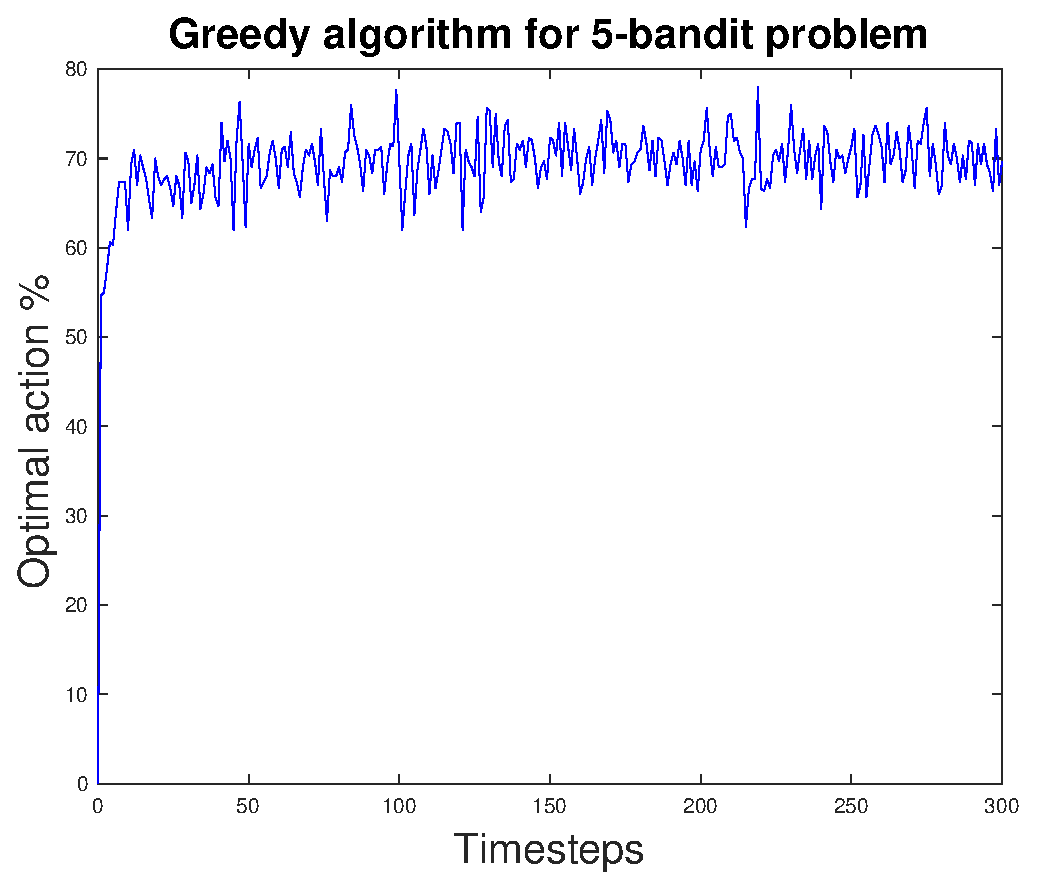
\includegraphics[width=\linewidth]{greedyplot2.eps}
			\captionof{figure}{Optimal action for greedy algorithm}
		\end{Figure}
		
		It can be observed above that the agent converges to the optimal action in around 70 percent of the bandit tasks. This simulation shows that although being very simple, the greedy algorithm shows an overall positive performance.
		
		\subsection{$\epsilon$-Greedy}
		\subsubsection{Theory}
		From the previous subsection, the theory and implementation of the greedy algorithm were shown. In this section, a variation of the greedy algorithm called $\epsilon$-Greedy will be explored. One of the issues from the $\epsilon$-Greedy was that because it always forced the agent to choose the best action-value in every state, if a particular action-value was low from the start, the agent never chose it for the rest of the simulation, therefore, never being able to discover its \textit{actual} value. To avoid this problem, a variant of this algorithm that allows the agent to \textit{explore} from time to time can be used. In every state, the agent will randomly choose an action with equal probability in all of them. This means that because if an action is chosen infinite times it converges to its textit{actual} value, this will allow the agent to have a more precise information of its options. This algorithm is called $\epsilon$-Greedy.
		
		\subsubsection{Simulation}
		The first simulation was created by using an $\epsilon$ of 0.1. The 5-bandit problem was run for 600 steps and averaged over 300 tasks. The result was then compared to the optimal return. This can be seen in the figure below.
		
		\begin{Figure}
			\centering
			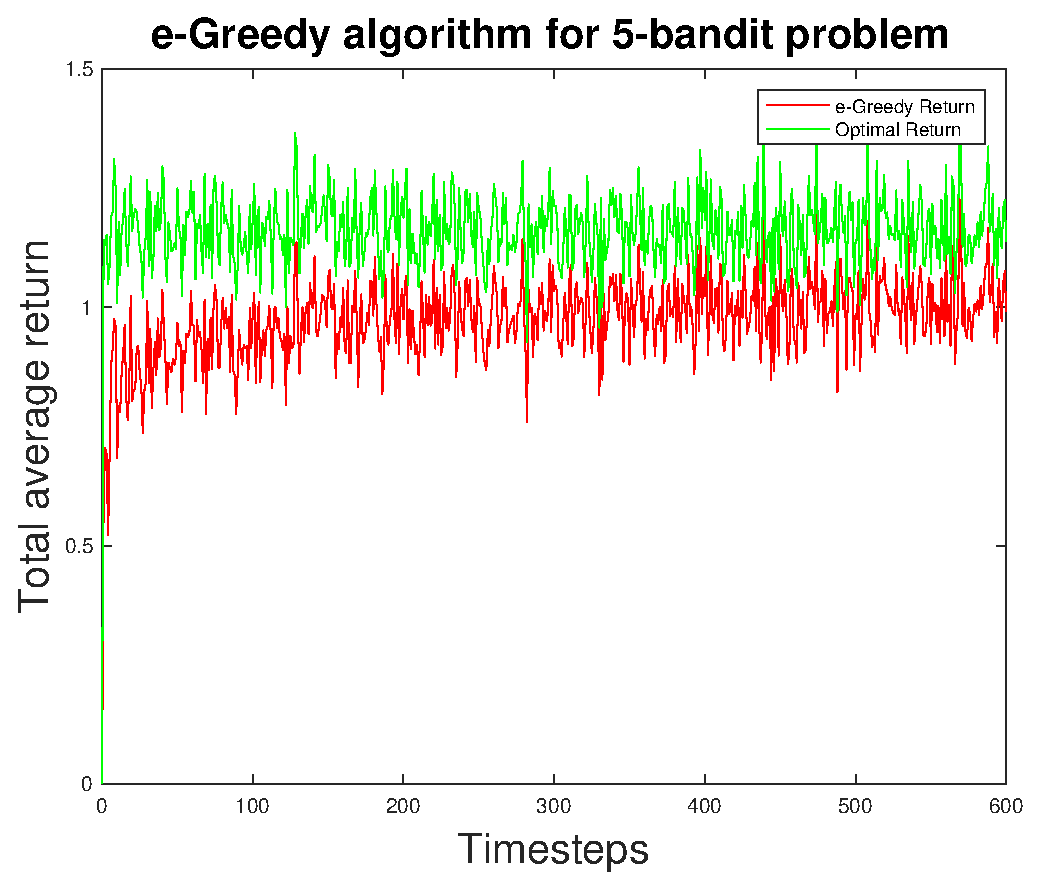
\includegraphics[width=\linewidth]{egreedyplot1.eps}
			\captionof{figure}{e-Greedy vs Optimal ($\epsilon$  = 0.1)}
		\end{Figure}
		
		From the graph above, we can see that opposed to the greedy algorithm, the average reward gets closer to the optimal average reward as the number of steps increases. In theory, as the number of steps goes to infinity, the average reward would converge to the optimal reward. \\
		
		Following this, a plot showing the percentage in which the agent converged to choose the optimal value is shown below.
		
		\begin{Figure}
			\centering
			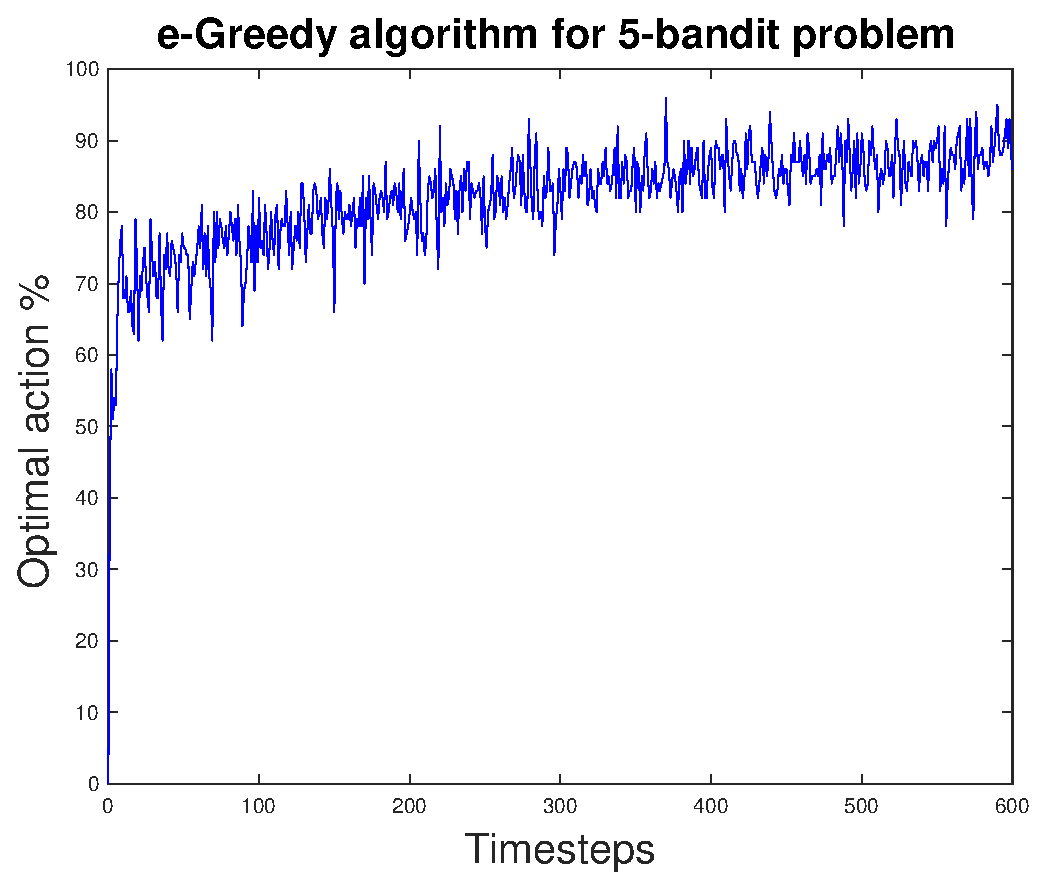
\includegraphics[width=\linewidth]{egreedyplot2.eps}
			\captionof{figure}{Optimal action for e-greedy algorithm ($\epsilon$  = 0.1)}
		\end{Figure}
		
		From analyzing the graph above, we can see that as we reach step 600, the optimal action percentage reaches around 90 percent. This is because we allow the agent to explore for 10 percent of the time. This means that although 10 percent of the time the action might not receive the maximum immediate reward, it will aid the agent to get a more precise estimate of the real value. \\
		
		For the last e-greedy simulation, an epsilon value of 0.01 was used. The first simulation compares the average return of this particular e-greedy algorithm against the optimal return.
		
		\begin{Figure}
			\centering
			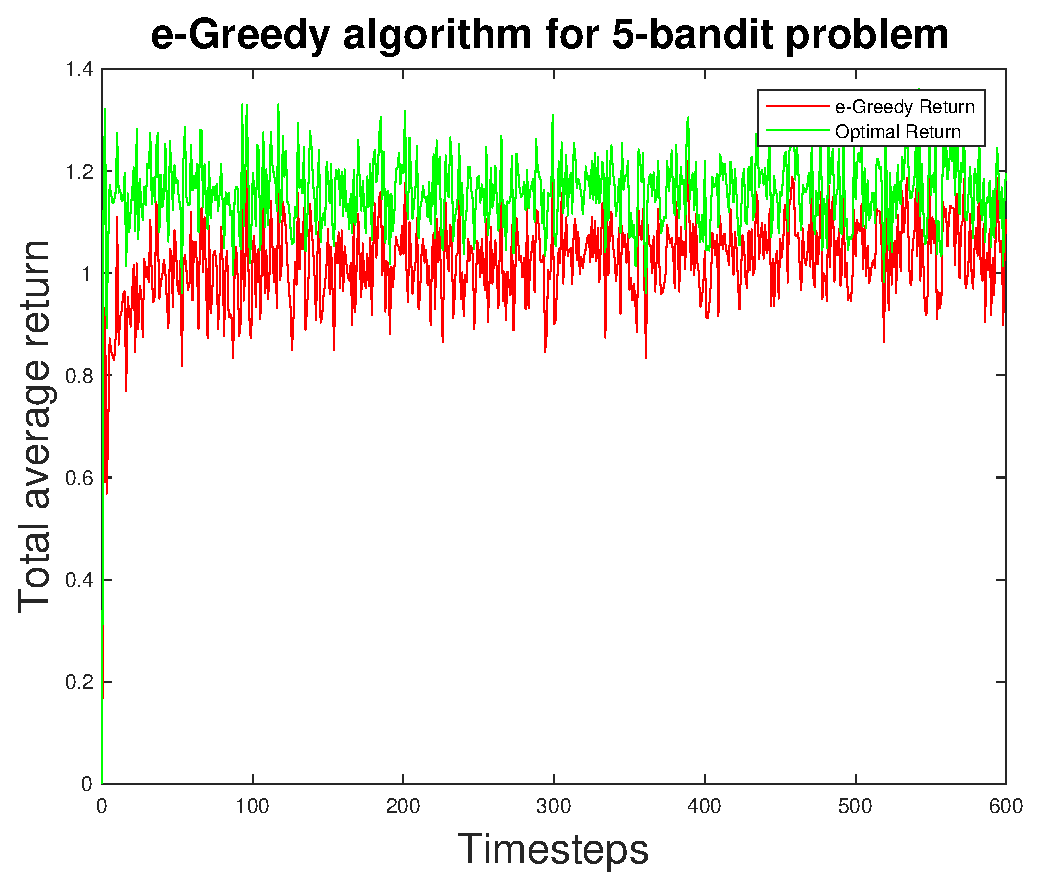
\includegraphics[width=\linewidth]{egreedyplot3.eps}
			\captionof{figure}{e-Greedy vs Optimal ($\epsilon$  = 0.01)}
		\end{Figure}
		
		From this graph, we can see that the average return increases steadily. If the number of steps is increased, this version of the e-greedy algorithm will outperform the other ones and eventually converge to an accuracy of optimal action to 99.9 percent.
		
		\begin{Figure}
			\centering
			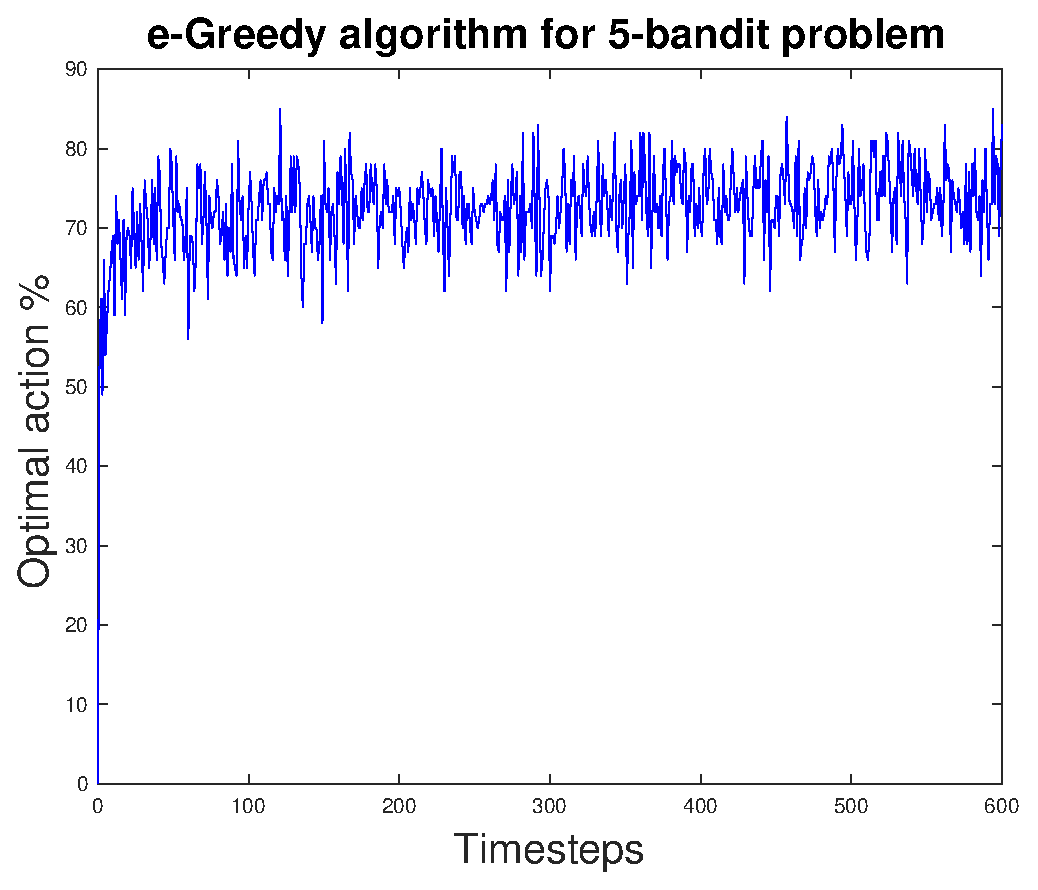
\includegraphics[width=\linewidth]{egreedyplot4.eps}
			\captionof{figure}{Optimal action for e-greedy algorithm ($\epsilon$  = 0.01)}
		\end{Figure}
	
		A more helpful graph is plotted above and show how how the optimal action percentage is steadily increased. Although is not as fast as using an epsilon 0.1, again, in the long run this configuration will outperform the previous configuration.
		
		\section{Dynamic Programming}
		\subsection{Policy Evaluation}
		The idea behind policy evaluation is to find the state-value for all the possible states using an arbitrary policy $\pi$. To compute the state-value we use one of Bellman's equations:
		
		\begin{equation}
			v_{k+1}(s) = \mathbf{E}_\pi[R_{t+1} + \gamma v_k(S_{t+1}) | S_t = s]
		\end{equation}
		
		This equation computes the estimated state-value for the following time step using information from the current state. This method is called full back up, because it uses the information in the values of all the available states to estimate a state-value.
		
		\subsection{Policy Iteration}
		In order to converge to the $v_\pi$ of each state we can iterate over the episodic system many times. This concept is called \textit{policy iteration}.
		
		\subsubsection{Gridworld example}
		Policy iteration can be applied in the gridworld scenario.
		
		
		
		
		\end{multicols}
		\pagebreak
	
		% Start of APPENDIX
		\begin{appendices}
		\chapter{Greedy function MATLAB code}
			\lstinputlisting{greedy.m}
		\chapter{e-Greedy function MATLAB code}
			\lstinputlisting{egreedy.m}
		\end{appendices}
\end{document}











